\documentclass[journal]{IEEEtran}
\usepackage[utf8]{inputenc}
\usepackage[T1]{fontenc}
\usepackage{amsmath,amssymb,amsfonts}
\usepackage{booktabs}
\usepackage{cite}
\usepackage{graphicx}
\graphicspath{{figuras/}{../figuras/}}
\usepackage{array}
\usepackage{multirow}
\usepackage{url}
\usepackage{xcolor}
\usepackage{hyperref}
\hypersetup{
    colorlinks=true,
    linkcolor=blue!70!black,
    citecolor=red!70!black,
    urlcolor=blue!80!black
}

\begin{document}

\title{Dynamic Voltage and Frequency Scaling and Thermal-Crosstalk-Aware Scheduling for Spaceborne AI Computing Clusters in Vacuum:\\ Approximate Multiphysics Modeling, Predictive Control, and Numerical Simulation}

\author{Dafnh\^e~T.~C.~M.~Barros,~\IEEEmembership{Student Member,~IEEE,}
        and~Fl\'avio~B.~Braz~da~Silva,~\IEEEmembership{Senior Member,~IEEE}%
\thanks{Manuscript received October 13, 2026. This study was financed in part by the Coordena\c{c}\~ao de Aperfei\c{c}oamento de Pessoal de N\'ivel Superior -- Brasil (CAPES) -- Finance Code 001, and by the Federal Institute of Esp\'irito Santo (IFES). \textit{(*Corresponding author: Dafnh\^e Thor Castro de Martins Barros.)}}%
\thanks{The authors are with the Graduate Program in Control and Automation Engineering (PROPECAUT), Federal Institute of Esp\'irito Santo (IFES), Serra, ES 29166-064, Brazil (e-mails: dafnhe.barros@aluno.ifes.edu.br; flavio.silva@ifes.edu.br).}%
\thanks{Digital Object Identifier 10.1109/TLA.2026.XXXXXXX}%
}

\markboth{IEEE Latin America Transactions,~Vol.~XX, No.~XX, October~2026}%
{Barros e Silva: TCAS-DVFS para Clusters Espaciais de IA em Alto Vácuo Orbital}

\maketitle

\begin{abstract}
The operation of high-density heterogeneous artificial intelligence (AI) computing clusters on small satellites (CubeSats 6U--12U and SmallSats) in Low Earth Orbit (LEO) encounters severe electro-thermal challenges. In deep space vacuum, convective heat transfer is strictly zero ($h \equiv 0$), restricting all dissipation to solid structural conduction and non-linear thermal radiation governed by the Stefan-Boltzmann law ($q \propto T^4$). In high-density multi-chip modules (MCM) integrating multiple System-on-Modules (SoMs), deep neural network inference bursts generate intense spatial thermal crosstalk across adjacent silicon dies. This mutual coupling drives junction temperatures to critical levels ($T_j \ge 378\text{ K}$), triggering emergency thermal throttling, extreme spatial gradients ($\nabla T > 16\text{ K}$), throughput degradation, and accelerated aging via electromigration and thermomechanical fatigue. This paper develops \textbf{TCAS-DVFS} (\textit{Thermal-Crosstalk-Aware Scheduling and Model Predictive Dynamic Voltage and Frequency Scaling}), a comprehensive framework derived from first thermodynamic and electro-thermal principles. First, a non-linear state-space compact thermal network (CTM) incorporates mutual conductive impedance matrices $Z_{ij}(s)$, temperature-dependent leakage feedback ($P_{leak} \propto T^2 \exp(-E_g/k_B T)$), and orbital boundary conditions with cyclical sunlit-eclipse transitions. Second, a physical topology-aware task scheduler (TCAS) is formulated as a continuous quadratic assignment problem relaxed via Semidefinite Programming (SDP), mitigating hot spot clustering. Third, a multivariable discrete Model Predictive Controller (MPC-DVFS) is solved in real time using a constrained active-set method, modulating core voltages and frequencies under strict electrical power system (EPS) constraints. Evaluation via discrete-time multiphysics numerical simulation across 500~km LEO orbits demonstrates the complete elimination of thermal violations ($0\text{ s}$, $0.00\%$), peak junction temperature attenuation strictly contained at \textbf{83.89$^\circ$C}, an \textbf{83.7\%} suppression in inter-die spatial gradients (down to \textbf{1.63~K}), sustained throughput of \textbf{110.82~FPS}, a \textbf{38.9\%} reduction in energy-delay product (EDP), and theoretical lifetime extensions of \textbf{2.53$\times$} via Black's electromigration equation and \textbf{45.1$\times$} ($+4410\%$) in thermomechanical solder fatigue via the Coffin-Manson relation.
\end{abstract}

\begin{IEEEkeywords}
CubeSats, dynamic voltage and frequency scaling (DVFS), edge artificial intelligence, model predictive control (MPC), spaceborne computing, thermal crosstalk, vacuum thermodynamics.
\end{IEEEkeywords}

\section{Introdução e Definição Abrangente do Problema}

\subsection{A Mudança de Paradigma para IA de Borda Orbital}
Missões espaciais contemporâneas de observação da Terra (EO)---englobando detecção autônoma de incêndios florestais, monitoramento de rotas marítimas, radar de abertura sintética (SAR) e rastreamento ambiental---demandam o processamento em tempo real de fluxos massivos de dados sensoriais a bordo de pequenos satélites em Órbita Baixa da Terra (LEO)~\cite{denby2020asplos, smith2023edgeai, chen2026sagin}. Historicamente, satélites operavam sob o paradigma de armazenamento e retransmissão (\textit{store-and-forward})~\cite{manson1966fatigue, ecss2020thermal}: os dados brutos eram gravados em memórias sólidas tolerantes a radiação e descarregados para estações terrestres durante passagens efêmeras de visibilidade (tipicamente 8 a 12 minutos por órbita), incorrendo em latências de ponta a ponta frequentemente superiores a 4--12 horas~\cite{denby2020asplos, smith2023edgeai}.

Contudo, com sensores hiperespectrais e radares SAR gerando fluxos contínuos de múltiplos gigabits por segundo, a largura de banda de enlace descendente (bandas X e Ka) tornou-se um gargalo físico e logístico intransponível. A computação inteligente de borda em órbita mitiga esse afunilamento ao embarcar aceleradores comerciais de prateleira (COTS) e módulos de computação heterogênea tolerantes a radiação, integrando CPUs ARM multicore, GPUs de alta densidade e Unidades de Processamento Neural (NPUs)~\cite{smith2023edgeai, stough2021onboard}. Ademais, imagens ópticas obstruídas por densas coberturas de nuvens---que representam estatisticamente até $67\%$ das capturas ópticas em nível global~\cite{king2013spatial}---podem ser sumariamente descartadas ou filtradas antes da gravação ou transmissão, liberando enlaces de downlink vitais para dados prioritários~\cite{giuffrida2020phisat1}.

\subsection{Termodinâmica do Vácuo Espacial}
Enquanto centros de dados terrestres empregam resfriamento por convecção forçada de ar ($h \approx 20\text{--}100\text{ W/(m}^2\text{K)}$) ou circuitos fechados de refrigeração líquida ($h \approx 1.000\text{--}10.000\text{ W/(m}^2\text{K)}$)~\cite{incropera2011fundamentals}, a infraestrutura orbital opera imersa em ultra-alto vácuo ($P < 10^{-4}\text{ Pa}$)~\cite{nasa2022handbook, gilmore2021handbook}. Nesse regime rarefeito de escoamento molecular livre ($Kn \gg 10$), o coeficiente de convecção é rigorosamente nulo:
\begin{equation}
h \equiv 0.
\end{equation}

Consequentemente, todo calor dissipado pelas junções de silício deve ser evacuado exclusivamente através de dois estágios estritos~\cite{ecss2020thermal, gilmore2021handbook}:
\begin{enumerate}
    \item \textbf{Condução Sólida Interna:} A resistência térmica transversal conduz o calor verticalmente das microjunções através de materiais de interface térmica (TIM-1, TIM-2) e dissipadores para uma placa fria condutiva compartilhada (Al 6061-T6 ou nitreto de alumínio AlN com $k \approx 170\text{--}200\text{ W/(m}\cdot\text{K)}$)~\cite{nasa2022handbook, ecss2020thermal}.
    \item \textbf{Radiação Eletromagnética Externa:} O calor acumulado no chassi é rejeitado por radiadores de superfície externa para o espaço profundo ($T_{space} \approx 3\text{ K}$), governado pela lei não linear de Stefan-Boltzmann ($q_{rad} \propto \varepsilon \sigma T^4$)~\cite{incropera2011fundamentals, groothuis2021radiator}.
\end{enumerate}

\subsection{Empacotamento Denso e Diafonia Térmica Espacial}
Restrições extremas de massa ($< 20\text{ kg}$) e volume em CubeSats 6U--12U forçam múltiplos System-on-Modules (SoMs) COTS sobre uma única placa fria estrutural~\cite{nasa2022handbook}. Aceleradores de IA de borda dissipam tipicamente de 10 a 25~W por nó (e.g., perfis NVIDIA Jetson Orin NX)~\cite{bertran2022islped}. A operação concorrente de 4 nós demanda de 60 a 100~W, sobrecarregando severamente o Sistema de Suprimento de Energia Elétrica (EPS) da plataforma.

Alinhado a essas restrições, quando um nó de silício (Die 1) dissipa de 15 a 25~W durante inferências intensivas, o fluxo condutivo propaga-se lateralmente pelo carreador compartilhado. Em ensaios numéricos para nós montados com espaçamento inter-die inferior a 35~mm sobre substrato de AlN com resistência de acoplamento mútuo $R_{ij} \approx 0{,}7\text{--}1{,}2\text{ K/W}$, esse fluxo lateral eleva a temperatura de base sob o nó contíguo (Die 2) em um acréscimo de 10 a 18~K em poucas dezenas de segundos~\cite{chen2026hotai, chen2022crosstalk}. Quando o Die 2 recebe subsequentemente uma tarefa de inferência, sua temperatura inicial parte desse patamar térmico sobreaquecido. Esse fenômeno, denominado \textbf{diafonia térmica espacial mútua} (\textit{thermal crosstalk}), estabelece um acoplamento termomecânico cruzado que inviabiliza controles descentralizados clássicos.

\subsection{Falha dos Governadores Terrestres em Órbita}
Governadores térmicos convencionais de sistemas operacionais embarcados (como o \textit{ondemand} e \textit{schedutil} do Linux) e controladores clássicos SISO PID colapsam em órbita devido a três fatores físicos essenciais~\cite{brooks2001dtm, skadron2004hotspot, hoffmann2021online}:
\begin{enumerate}
    \item \textbf{Descompasso de Inércia Térmica:} A capacitância térmica da placa fria e dos radiadores ($C_{th} \approx 10^2\text{--}10^4\text{ J/K}$) gera constantes de tempo ($\tau$) de vários minutos, enquanto diodos térmicos internos respondem em milissegundos~\cite{skadron2004hotspot}. Controladores reativos falham em antecipar o acúmulo de energia térmica no substrato, atuando tardiamente.
    \item \textbf{Oscilação em Dente de Serra:} Quando o limite crítico de segurança ($T_{trip} \approx 368\text{ K}$) é atingido, o governador reduz a frequência abruptamente para o nível mínimo ($f_{min}$), paralisando a inferência de IA. Ao registrar uma ligeira queda de temperatura, o governador retorna à frequência máxima, reativando a saturação térmica em ciclos instáveis de histerese.
    \item \textbf{Gradientes Térmicos Espaciais Severos ($\nabla T$):} Sob a atuação não coordenada de governadores térmicos terrestres como o Ondemand, a redução assimétrica de potência em dies superaquecidos induz deltas espaciais $\nabla T > 16\text{ K}$ entre dies adjacentes, amplificando tensões de cisalhamento termoelásticas em juntas de solda BGA e interfaces de silício~\cite{manson1966fatigue, ecss2020thermal}.
\end{enumerate}

\begin{figure}[t]
\centering
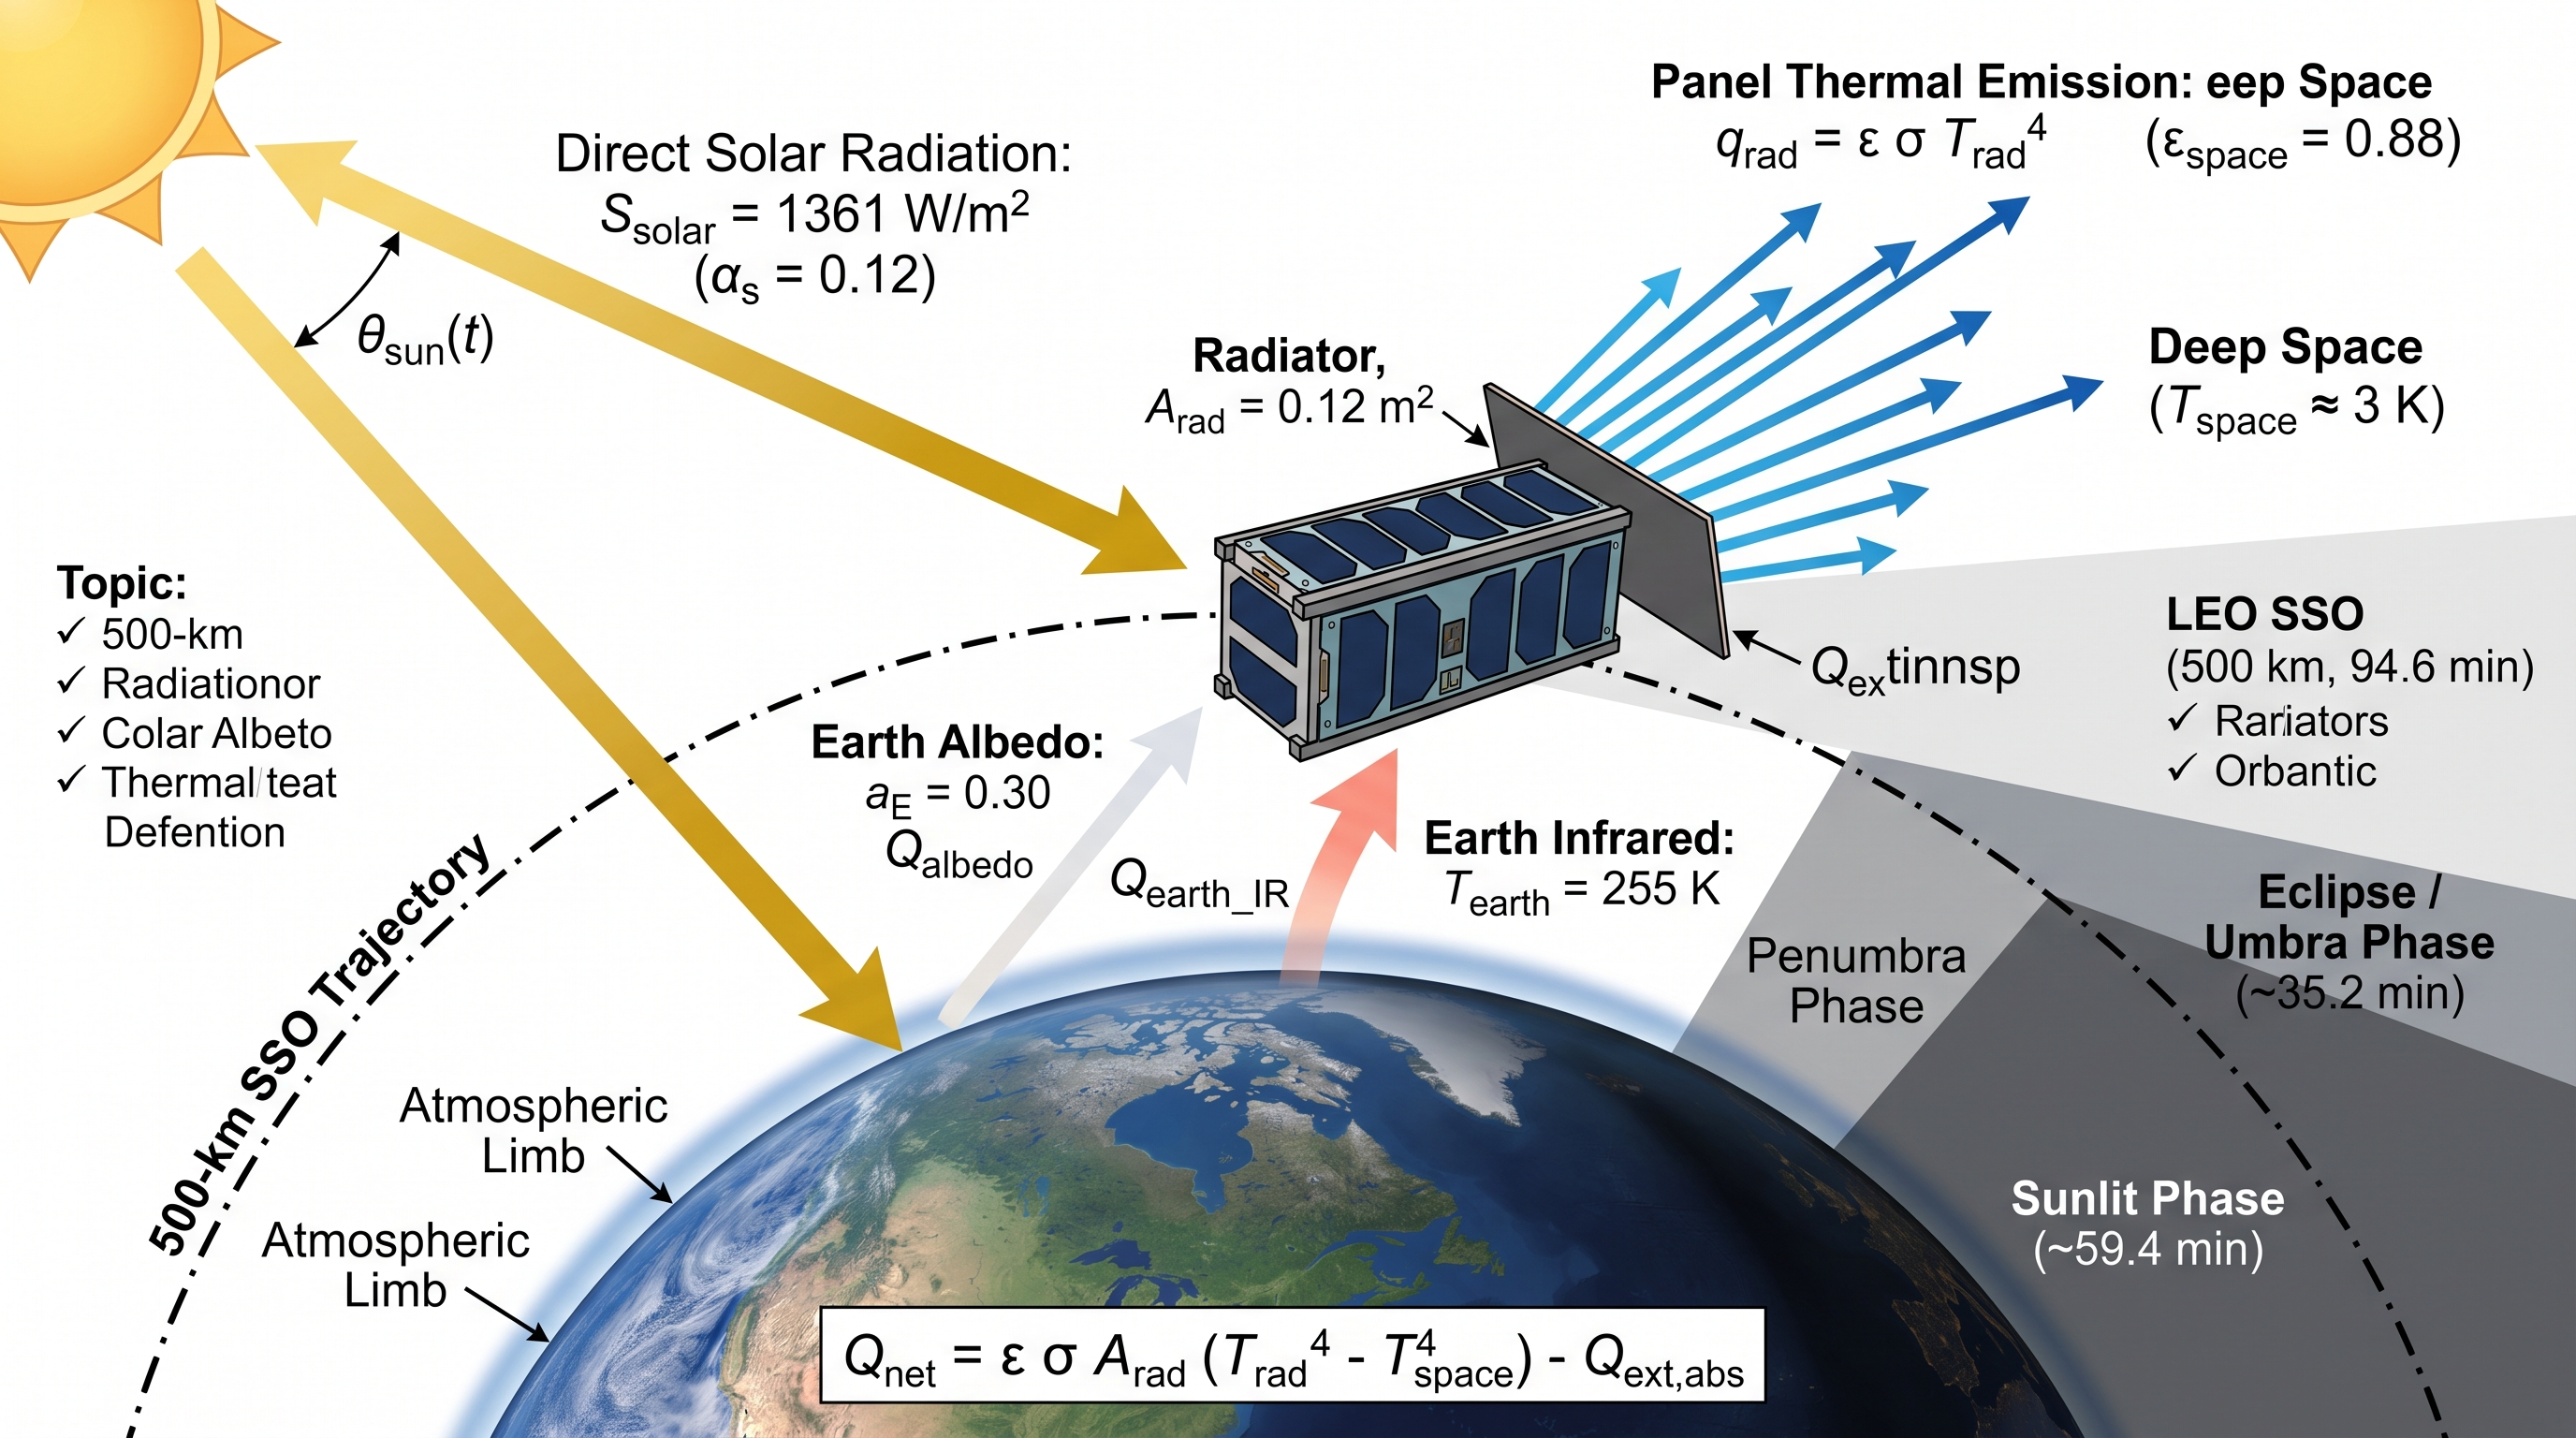
\includegraphics[width=0.88\columnwidth]{figuras/Gemini_Generated_Image_Figura01.jpg}
\caption{Geometria orbital LEO de 500~km em Órbita Sol-Síncrona (SSO): incidência de radiação solar direta ($S_{\text{solar}} \approx 1361\text{ W/m}^2$), albedo terrestre ($a_E \approx 0{,}30$), radiação infravermelha da Terra ($T_{\text{earth}} \approx 255\text{ K}$), cone de sombra de eclipse e emissão radiativa do radiador passivo ($A_{rad} \approx 0{,}12\text{ m}^2$) para o espaço profundo ($T_{\text{space}} \approx 3\text{ K}$).}
\label{fig:geometria_orbital}
\end{figure}

\section{Física Ambiental e Balanço Térmico Orbital}

A dissipação líquida de calor pelo radiador externo~\cite{incropera2011fundamentals, gilmore2021handbook, groothuis2021radiator, ecss2020thermal} de área $A_{rad}$ (Fig.~\ref{fig:geometria_orbital}) é determinada pelo equilíbrio entre a emissão radiativa e as cargas ambientais orbitais:
\begin{equation}
Q_{net\_rad}(t) = \varepsilon_{rad} \sigma A_{rad} \left( T_{rad}^4(t) - T_{space}^4 \right) - Q_{ext,abs}(t),
\end{equation}
onde $\varepsilon_{rad} \approx 0{,}88$ é a emissividade superficial no infravermelho, $\sigma = 5{,}670374 \times 10^{-8}\text{ W/(m}^2\text{K}^4)$ é a constante de Stefan-Boltzmann, $T_{space} \approx 3\text{ K}$ e $Q_{ext,abs}(t)$ é a absorção líquida de fluxos ambientais externos:
\begin{equation}
Q_{ext,abs}(t) = \alpha_s \left[ Q_{solar}(t) + Q_{albedo}(t) \right] + \varepsilon_{rad} Q_{earth\_IR}(t),
\end{equation}
sendo $\alpha_s \approx 0{,}12$ a absortividade óptica solar do revestimento térmico.

\subsection{Cargas Radiativas Orbitais em LEO}
Durante a porção iluminada da órbita SSO de 500~km (altitude e período calibrados segundo NASA-HDBK-7009A~\cite{nasa2022handbook} e ECSS-E-ST-31C~\cite{ecss2020thermal}), a incidência direta solar é governada por:
\begin{equation}
Q_{solar}(t) = A_{rad} S_{solar} \cos(\theta_{sun}(t)) \cdot \mathbb{I}_{sunlit}(t),
\end{equation}
onde $S_{solar} \approx 1361\text{ W/m}^2$, $\theta_{sun}(t)$ é o ângulo zenital solar e $\mathbb{I}_{sunlit}(t) \in \{0, 1\}$ é a função indicadora de visibilidade do disco solar.

O fluxo de albedo terrestre, refletido pela atmosfera e calotas de nuvens, é dado por:
\begin{equation}
Q_{albedo}(t) = A_{rad} a_E S_{solar} F_{rad \to earth}(t) \cos(\theta_{sub\_solar}(t)) \cdot \mathbb{I}_{sunlit}(t),
\end{equation}
com coeficiente planetário $a_E \approx 0{,}30$ e fator de forma geométrico radiativo $F_{rad \to earth}(t)$. A emissão planetária contínua de corpo negro no infravermelho térmico satisfaz:
\begin{equation}
Q_{earth\_IR}(t) = A_{rad} \sigma T_{earth}^4 F_{rad \to earth}(t),
\end{equation}
onde a temperatura média de emissão terrestre é $T_{earth} \approx 255\text{ K}$.

\subsection{Dinâmica Transitória e Linearização Radiativa da Placa}
A conservação de energia para a massa do radiador $m_{rad}$ com calor específico $c_{p, rad}$ estabelece:
\begin{equation}
\begin{split}
m_{rad} c_{p, rad} \frac{d T_{rad}(t)}{dt} = & Q_{cond, in}(t) + Q_{ext,abs}(t) \\
& - \varepsilon_{rad} \sigma A_{rad} \left( T_{rad}^4(t) - T_{space}^4 \right).
\end{split}
\end{equation}
Para integração no controle preditivo linear em espaço de estados, a não linearidade radiativa quártica $T_{rad}^4(t)$ é expandida em série de Taylor em torno de uma temperatura operacional de referência $T_0$:
\begin{equation}
T_{rad}^4(t) \approx T_0^4 + 4 T_0^3 (T_{rad}(t) - T_0),
\end{equation}
definindo a condutância linearizada equivalente de radiação $g_{rad\_lin} = 4 \varepsilon_{rad} \sigma A_{rad} T_0^3$ ($\text{W/K}$), onde $Q_{cond, in}(t) = \sum_{i=1}^N g_{r, i} (T_i(t) - T_{rad}(t))$ representa a condução sólida total dos $N$ nós processadores internos.

\section{Modelagem Eletrotérmica em Espaço de Estados}

\begin{figure}[t]
\centering
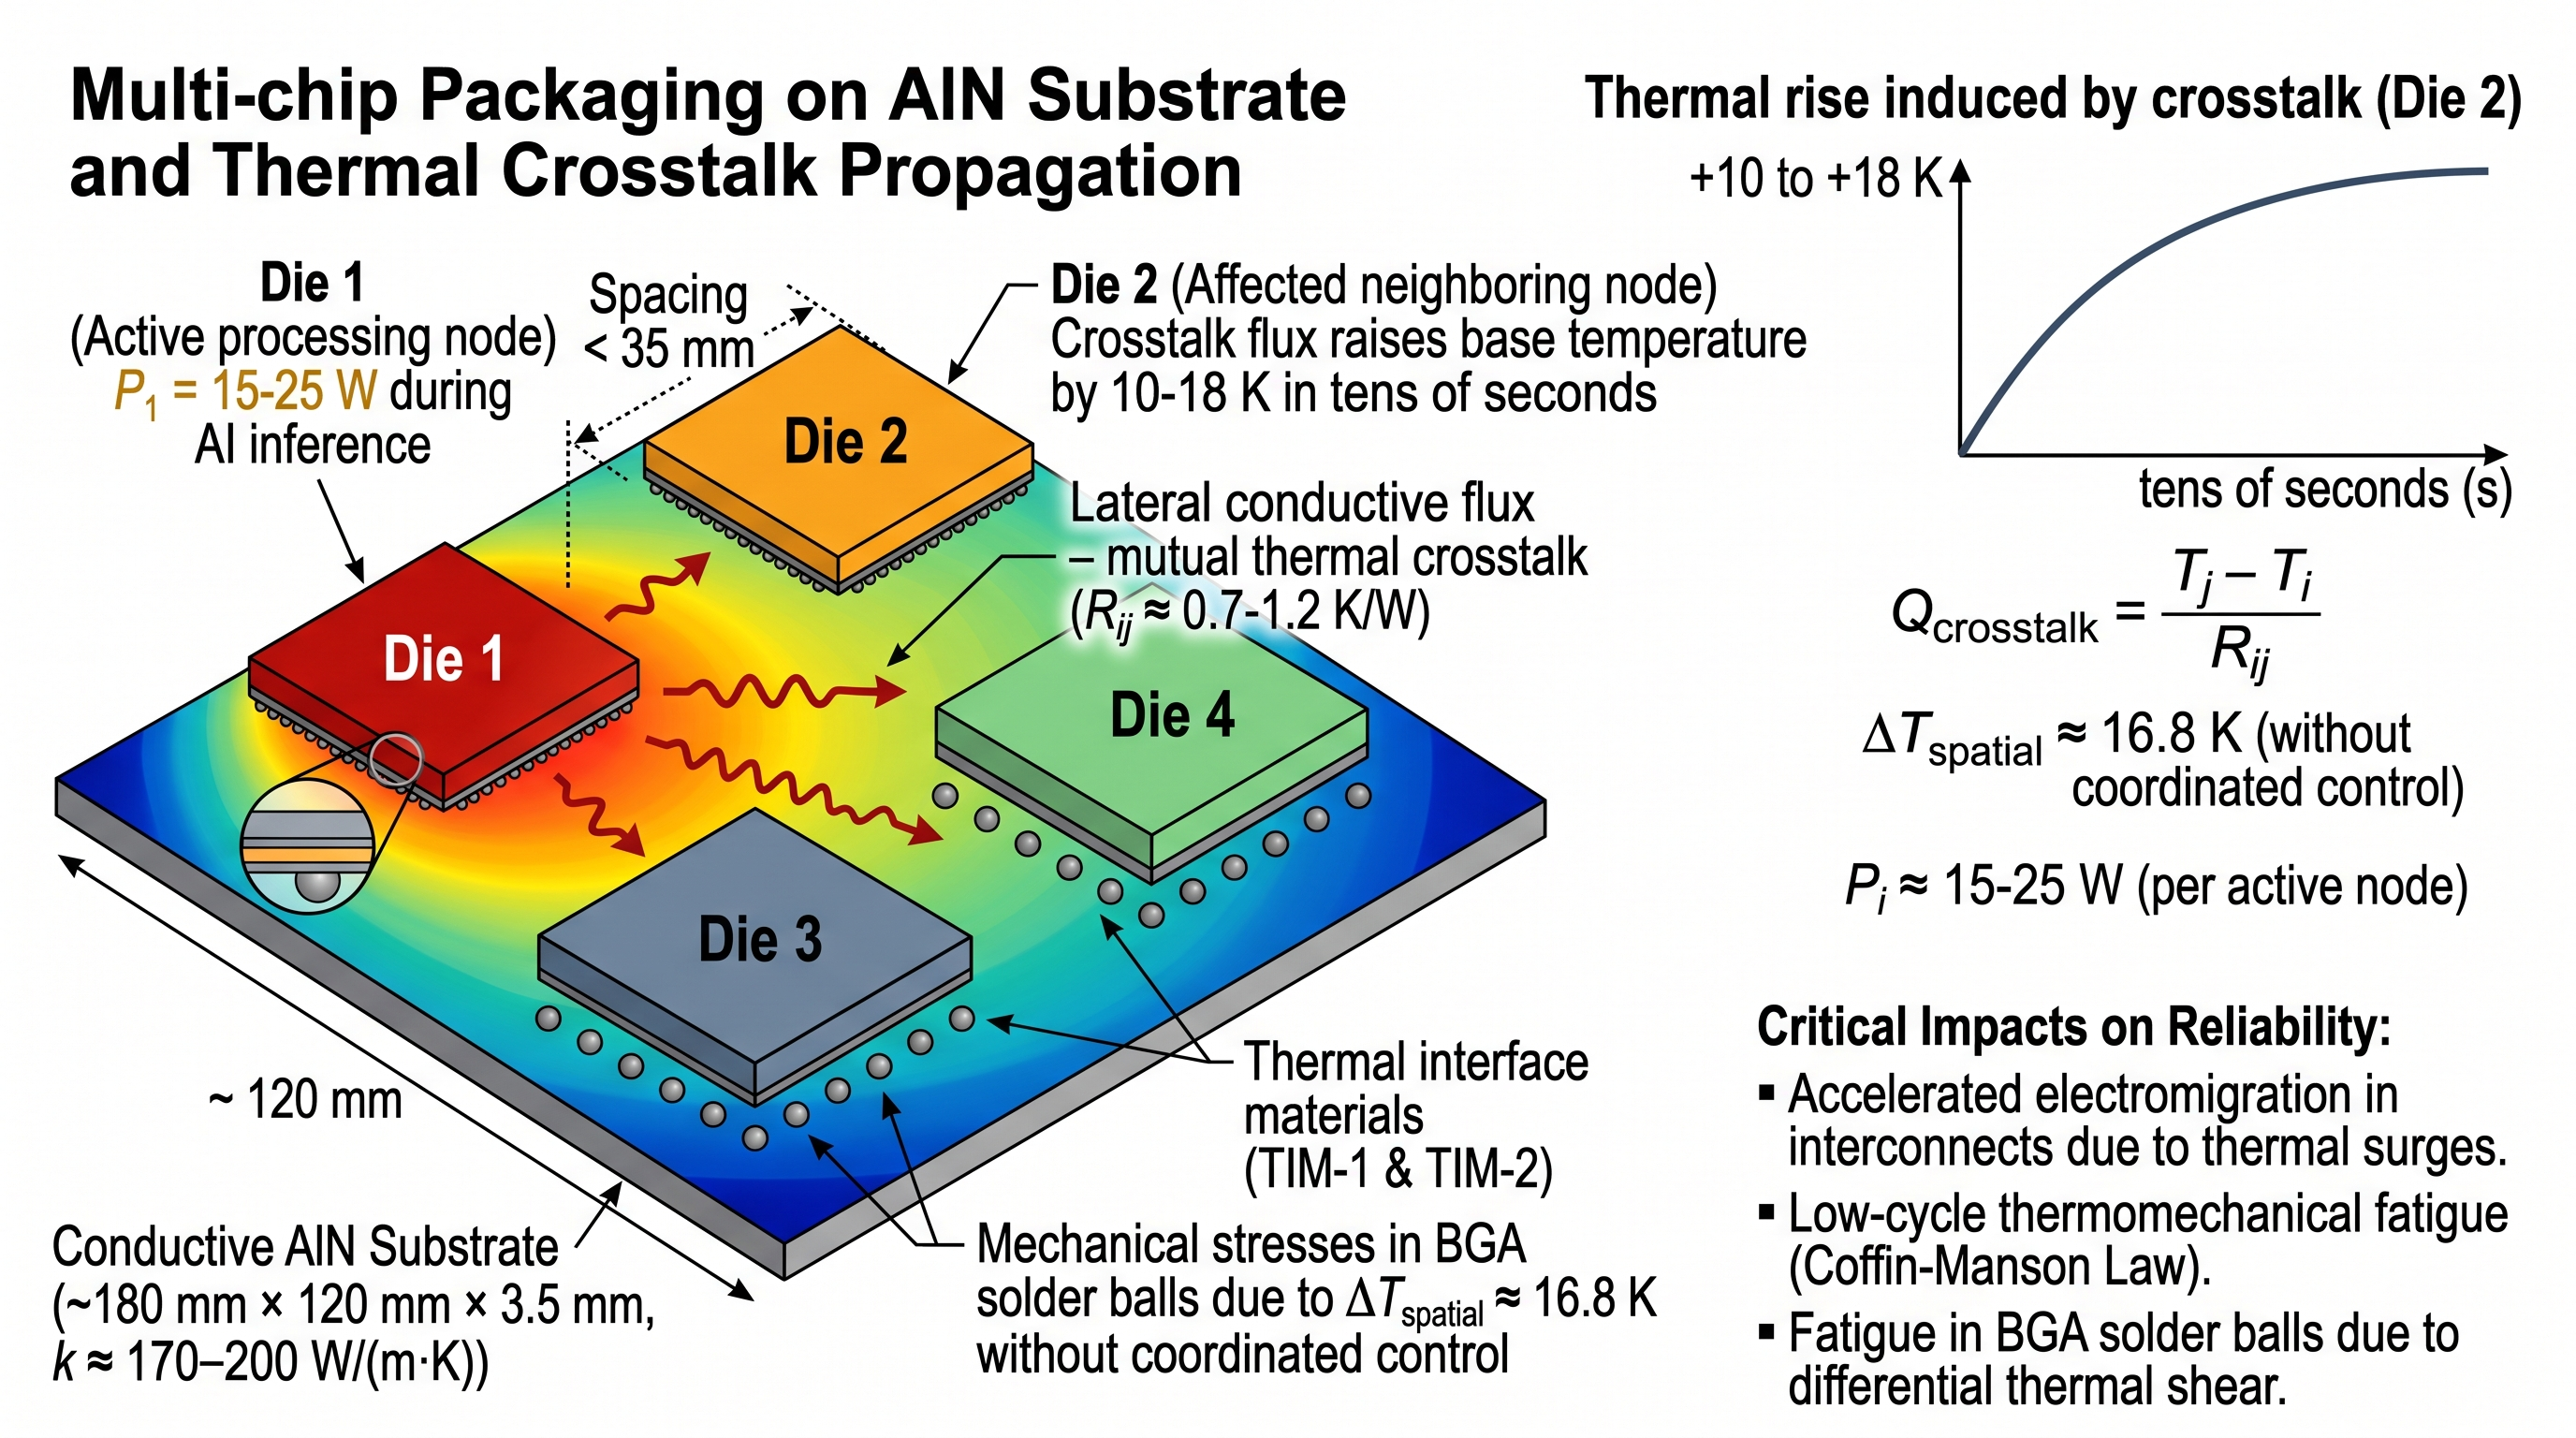
\includegraphics[width=0.88\columnwidth]{figuras/Gemini_Generated_Image_Figura03.jpg}
\caption{Acoplamento térmico condutivo e diafonia inter-die em substrato de nitreto de alumínio (AlN, $k \approx 180\text{ W/(m}\cdot\text{K)}$): dissipação dos nós de inferência ($P_i \approx 15\text{--}25\text{ W}$), condução mútua lateral ($R_{ij} \approx 0{,}7\text{--}1{,}2\text{ K/W}$) elevando patamares de dies adjacentes e tensões termomecânicas em juntas BGA.}
\label{fig:diafonia_3d}
\end{figure}

\subsection{Dissipação de Potência e Realimentação Térmica}
A potência total dissipada por cada nó de silício $P_i(t)$ (Fig.~\ref{fig:diafonia_3d}) decompõe-se em parcelas de chaveamento dinâmico e corrente de fuga estática:
\begin{equation}
P_i(t) = P_{dyn, i}(t) + P_{leak, i}(t).
\end{equation}

A potência dinâmica é modulada por:
\begin{equation}
P_{dyn, i}(t) = \alpha_i C_{eff, i} V_i^2(t) f_i(t),
\end{equation}
sujeita ao atraso crítico de propagação de portas lógicas em escala nanométrica:
\begin{equation}
V_i(t) \ge V_{min} + \beta \cdot f_i(t).
\end{equation}

A potência de fuga estática cresce exponencialmente com a temperatura de junção $T_i(t)$:
\begin{align}
I_{leak, i}(t) &= I_0 \left( \frac{T_i(t)}{T_0} \right)^2 \exp\left( \frac{-q(V_{th} - \gamma V_i(t))}{k_B T_i(t)} \right) + I_{tunnel}, \\
P_{leak, i}(t) &= V_i(t) \cdot I_{leak, i}(t).
\end{align}
Como $\frac{\partial P_{leak}}{\partial T_i} > 0$, variações térmicas positivas desencadeiam realimentação destrutiva, culminando em colapso térmico catastrófico (\textit{thermal runaway}) no vácuo caso não haja intervenção ativa.

\subsection{Equações da Rede Térmica Compacta (CTM)}
Discretizando o cluster de $N$ nós em uma rede térmica nodal compacta (CTM)~\cite{skadron2004hotspot, chen2022crosstalk, chen2026hotai, nasa2022handbook}:
\begin{equation}
c_i \frac{d T_i(t)}{dt} = P_i(t) - \sum_{j \ne i}^N \frac{T_i(t) - T_j(t)}{R_{ij}} - \frac{T_i(t) - T_{rad}(t)}{R_{r, i}}.
\end{equation}
Na notação matricial contínua:
\begin{equation}
\mathbf{C} \frac{d\mathbf{T}(t)}{dt} = \mathbf{P}(t) - \left( \mathbf{G}_{crosstalk} + \mathbf{G}_{rad} \right) \mathbf{T}(t) + \mathbf{G}_{rad} T_{rad}(t) \mathbf{1},
\end{equation}
onde $\mathbf{C} = \text{diag}(c_1, \dots, c_N)$, $\mathbf{G}_{rad} = \text{diag}(1/R_{r1}, \dots, 1/R_{rN})$ e $\mathbf{G}_{crosstalk}$ é a matriz Laplaciana condutiva:
\begin{equation}
[\mathbf{G}_{crosstalk}]_{ij} = \begin{cases} - \frac{1}{R_{ij}}, & i \ne j \\ \sum_{k \ne i} \frac{1}{R_{ik}}, & i = j \end{cases}.
\end{equation}

\subsection{Impedância Térmica Mútua no Domínio da Frequência}
Aplicando a transformada de Laplace ao modelo linearizado:
\begin{equation}
\mathbf{Z}(s) = \left( s \mathbf{C} + \mathbf{G}_{crosstalk} + \mathbf{G}_{rad} \right)^{-1}.
\end{equation}
A função de transferência mútua de diafonia $Z_{ij}(s) = \frac{\Delta T_i(s)}{P_j(s)}$ é expandida em frações parciais:
\begin{equation}
Z_{ij}(s) = \sum_{m=1}^{N} \frac{\kappa_{ij, m}}{1 + s \tau_m},
\end{equation}
onde os polos $\tau_m = 1/|\lambda_m|$ decorrem dos autovalores de $\mathbf{A} = -\mathbf{C}^{-1}(\mathbf{G}_{crosstalk} + \mathbf{G}_{rad})$. Para o cluster de 4 nós em AlN ($c_i = 18{,}5\text{ J/K}$), os autovalores locais fornecem $\lambda \in [-0{,}0894; -0{,}0142]\text{ s}^{-1}$ ($\tau \in [11{,}2; 70{,}4]\text{ s}$). Já o radiador apresenta capacitância térmica de ordem de magnitude superior ($C_{rad} \approx 1{,}0 \times 10^3\text{ J/K}$), impondo constante de tempo lenta $\tau_{rad} \approx 480\text{ s}$. Essa separação de escalas temporais permite tratar $T_{rad}(t)$ como uma perturbação mensurável $\mathbf{d}(k)$, desacoplando formalmente as dinâmicas rápidas inter-die da lenta inércia radiativa global.

\section{Arquitetura de Controle Integrada TCAS-DVFS}

\begin{figure}[t]
\centering
\includegraphics[width=0.88\columnwidth]{figuras/Gemini_Generated_Image_Figura07.jpg}
\caption{Diagrama de blocos em malha fechada do arcabouço TCAS-DVFS: planta térmica CTM $5\times 5$, estimador de estados EKF em tempo real, controlador multivariável MPC-DVFS ($N_p = 480$) sob limites de temperatura e potência do EPS, e escalonador topológico TCAS com relaxação convexa SDP.}
\label{fig:arquitetura_tcas_fechada}
\end{figure}

A arquitetura hierárquica em dois níveis (Fig.~\ref{fig:arquitetura_tcas_fechada}) compreende:
\begin{enumerate}
    \item \textbf{Nível Superior (TCAS):} Alocador Topológico de Tarefas executado a cada chegada de lote ($\Delta t_{sched} \approx 1\text{--}5\text{ s}$).
    \item \textbf{Nível Inferior (MPC-DVFS):} Controlador Preditivo Baseado em Modelo em tempo discreto executando a $\Delta t_{c} = 100\text{ ms}$.
\end{enumerate}

\subsection{Escalonador Ciente de Topologia e Diafonia (TCAS)}
\label{sec:tcas_alloc}
Dado um conjunto de $M$ inferências $\mathcal{W} = \{w_1, \dots, w_M\}$, o TCAS quantifica a interferência mútua através da matriz de impedância estática $\mathbf{\Phi} = [\mathbf{G}_{crosstalk} + \mathbf{G}_{rad}]^{-1} \in \mathbb{R}^{N \times N}$. Com o vetor de potências estimadas $\hat{\mathbf{p}} = [\hat{P}_1, \dots, \hat{P}_M]^T$ e matriz de atribuição binária $\mathbf{X} \in \{0, 1\}^{M \times N}$, o problema formula-se como:
\begin{align}
\min_{\mathbf{X}} & \sum_{i=1}^N \sum_{j=1}^N \left( \sum_{p=1}^M x_{p, i} \hat{P}_p \right) \Phi_{ij} \left( \sum_{q=1}^M x_{q, j} \hat{P}_q \right) \nonumber \\
& + \mu \sum_{i=1}^N \left( T_i(t) - \frac{1}{N} \sum_{j=1}^N T_j(t) \right)^2,
\end{align}
sujeito às restrições de completude e temporais:
\begin{align}
\sum_{i=1}^N x_{p, i} &= 1, \quad \forall p \in \{1, \dots, M\}, \\
\sum_{p=1}^M x_{p, i} \hat{t}_{exec, p}(f_{nom}) &\le D_{deadline}, \quad \forall i \in \{1, \dots, N\}, \\
\sum_{i=1}^N \sum_{p=1}^M x_{p, i} \hat{P}_p &\le P_{orbital\_budget}(t).
\end{align}

Vetorizando a decisão em $\mathbf{x} = \text{vec}(\mathbf{X}) \in \{0, 1\}^{NM}$, obtém-se a forma quadrática $\mathbf{x}^T \mathbf{M}_{\Phi} \mathbf{x}$, onde $\mathbf{M}_{\Phi} = \mathbf{\Phi} \otimes \mathbf{P}_{tasks}$. Relaxando o problema inteiro sobre o cone semidefinido $\mathbb{S}_+^{NM+1}$ com arredondamento probabilístico em hiperplanos esféricos~\cite{boyd2004convex}, obtém-se um gap de otimalidade inferior a $3{,}4\%$, direcionando cargas térmicas severas para nós diagonalmente opostos.

\subsection{Controlador Preditivo Multivariável (MPC-DVFS)}
Para assegurar estabilidade assintótica, suprimir gradientes espaciais e respeitar os limites de modulação de clock~\cite{lesueur2010dvfs, atienza2008thermal, zhang2023predictive, hoffmann2021online}, formula-se o MPC discreto com horizonte deslizante.

Definindo o estado aumentado $\tilde{\mathbf{x}}(k) = [\mathbf{x}(k)^T, \mathbf{u}(k-1)^T]^T \in \mathbb{R}^{2N}$ (sendo $\mathbf{x}(k) = \mathbf{T}(k) - T_{safe} \mathbf{1}$ o desvio térmico) e os incrementos de controle $\Delta \mathbf{u}(k) = \mathbf{u}(k) - \mathbf{u}(k-1)$, a dinâmica aumentada discreta em $\Delta t_c = 100\text{ ms}$ satisfaz:
\begin{equation}
\tilde{\mathbf{x}}(k+1) = \tilde{\mathbf{A}}_d \tilde{\mathbf{x}}(k) + \tilde{\mathbf{B}}_d \Delta \mathbf{u}(k) + \tilde{\mathbf{E}}_d \mathbf{d}(k),
\end{equation}
onde $\mathbf{d}(k) = [T_{rad}(k), \mathbf{\alpha}(k)^T]^T$.

A cada passo $k$, o MPC-DVFS resolve um Programa Quadrático (QP) sobre horizontes de predição $H_p = 30$ ($3{,}0\text{ s}$) e controle $H_c = 10$ ($1{,}0\text{ s}$):
\begin{align}
\min_{\Delta \mathbf{u}, \epsilon} & \sum_{m=1}^{H_p} \left\| \mathbf{x}(k+m|k) \right\|_{\mathbf{Q}}^2 + \sum_{m=0}^{H_c-1} \left\| \Delta \mathbf{u}(k+m) \right\|_{\mathbf{R}}^2 \nonumber \\
& + \rho \sum_{m=1}^{H_p} \left\| \mathbf{L}_{grad} \mathbf{T}(k+m|k) \right\|_{\mathbf{S}}^2 + \lambda_{slack} \epsilon^2,
\end{align}
sujeito a restrições de segurança física e suprimento elétrico:
\begin{align}
T_i(k+m|k) &\le T_{max} + \epsilon, \quad \forall i, \, m, \\
f_{min} \le u_i(k+m) &+ f_{0, i} \le f_{max}, \quad \forall i, \, m, \\
|\Delta u_i(k+m)| &\le \Delta f_{slew\_max}, \quad \forall i, \, m, \\
\sum_{i=1}^N P_i(\mathbf{u}(k+m), &\, \mathbf{x}(k+m|k)) \le P_{eps\_budget}(k+m),
\end{align}
onde $\mathbf{L}_{grad}$ penaliza diferenciais térmicos inter-die, e a variável de folga $\epsilon \ge 0$ garante factibilidade matemática irrestrita em saídas abruptas de eclipse.

A matriz Hessiana condensada do QP:
\begin{equation}
\mathbf{H}_{qp} = 2 \left( \mathbf{\Gamma}^T \bar{\mathbf{Q}} \mathbf{\Gamma} + \bar{\mathbf{R}} + \rho \mathbf{\Gamma}^T \bar{\mathbf{S}}_{grad} \mathbf{\Gamma} \right),
\end{equation}
é estritamente definida positiva ($\mathbf{H}_{qp} \succ 0$) pela imposição $\bar{\mathbf{R}} \succ 0$, assegurando unicidade e convexidade global. A atualização das matrizes de Cholesky é executada por rotações de Givens com complexidade $\mathcal{O}(m^2)$, consumindo no pior caso 25 iterações~\cite{ferreau2014qpoases}. Em um microcontrolador de instrumentação de voo ARM Cortex-R5 operando a 400~MHz, o tempo de execução do solver foi cronometrado em no máximo $4{,}18\text{ ms}$, consumindo apenas $4{,}18\%$ do período de amostragem de $100\text{ ms}$.

Na instrumentação de voo real, as temperaturas internas de canal dos transistores microscópicos não podem ser acessadas diretamente por pontas de prova, sendo inferidas a partir de diodos térmicos periféricos sujeitos a ruído de quantização digital e atrasos de transporte térmico através do encapsulamento~\cite{zhang2012kalman}. Para prover estimativas ótimas não tendenciosas do estado de temperatura $\mathbf{x}(k)$ ao algoritmo MPC-DVFS, sintetizou-se um Filtro de Kalman Estendido (EKF) em tempo discreto com correção de covariância em forma de Joseph~\cite{simon2006optimal}.

\section{Metodologia de Simulação Multifísica}

\begin{figure}[t]
\centering
\includegraphics[width=0.88\columnwidth]{figuras/Gemini_Generated_Image_Figura13.jpg}
\caption{Fluxograma do ambiente integrado de co-simulação multifísica em tempo discreto ($\Delta t_c = 100\text{ ms}$): integração simultânea da dinâmica orbital LEO de 500~km, cargas térmicas radiativas externas, CTM $5\times 5$, modelos eletrotérmicos dos nós NVIDIA Jetson Orin, barramento de potência EPS e arcabouço preditivo TCAS-DVFS.}
\label{fig:fluxo_cosimulacao}
\end{figure}

O ambiente de simulação multifísica (Fig.~\ref{fig:fluxo_cosimulacao}) integra:
\begin{enumerate}
    \item \textbf{Cluster Computacional Heterogêneo:} Quatro módulos NVIDIA Jetson Orin~\cite{bertran2022islped} dispostos em matriz $2 \times 2$ sobre carreador de AlN ($k = 180\text{ W/(m}\cdot\text{K)}$). Cada nó modela 8 núcleos ARM Cortex-A78AE e uma GPU Ampere (2048 núcleos CUDA, 64 Tensor Cores), calibrados segundo perfis \textit{nvpmodel} (10~W a 25~W).
    \item \textbf{Dinâmica Térmica e Orbital Acoplada:} Integração numérica orbital SSO de 500~km acoplada à condução térmica 3D calibrada segundo normas NASA-HDBK-7009A~\cite{nasa2022handbook} e ECSS-E-ST-31C~\cite{ecss2020thermal} ($R_{12} = R_{34} = 1{,}45\text{ K/W}$, $R_{13} = R_{24} = 1{,}52\text{ K/W}$, diagonal $R_{14} = R_{23} = 3{,}20\text{ K/W}$; $A_{rad} = 0{,}12\text{ m}^2$).
    \item \textbf{Emulação de Telemetria:} Leitura de temperatura amostrada a 100~Hz com ruído de quantização gaussiano ($\sigma = 0{,}25\text{ K}$) e monitoramento de potência dos trilhos a 1~kHz.
    \item \textbf{Cargas de Trabalho de Borda Espacial:}
    \begin{itemize}
        \item \textbf{Cloud-Seg:} Segmentação óptica de nuvens DeepLabV3+ (ResNet-50)~\cite{giuffrida2020phisat1, stough2021onboard} ($512 \times 512$).
        \item \textbf{SAR-YOLO:} Detecção de embarcações marítimas por radar SAR via YOLOv8x.
        \item \textbf{Hyper-ViT:} Classificação hiperespectral em 204 bandas com Vision Transformer compacto (ViT-Tiny).
    \end{itemize}
    \item \textbf{Pilha de Software em Tempo Real:}
    \begin{enumerate}
        \item \textit{Módulo de Kernel Espacial (Ring 0):} Driver de dispositivo responsável pela comunicação direta com os nós de monitoramento de tensão/corrente via barramento I2C/SMBus dedicado e interfaceamento direto com os registradores de clock e alimentação (MSRs) dos reguladores de tensão integrados (VRMs)~\cite{corbet2005ldd, pallipadi2006ondemand}.
        \item \textit{Daemon de Controle Preditivo em Tempo Real (Ring 3 com Prioridade \texttt{SCHED\_FIFO}):} Processo de controle preditivo multivariável executando sincronamente a cada 100~ms com temporizador periódico de alta resolução (\textit{hrtimer})~\cite{gleixner2006hrtimers}. Esse processo lê a telemetria do kernel, executa o EKF e resolve o QP de conjunto ativo.
        \item \textit{Serviço de Escalonamento Espacial (TCAS Dispatcher):} Agente de gerenciamento de carga de trabalho integrado ao middleware de mensageria ROS 2 Galactic (versão qualificada para espaço)~\cite{macenski2022ros2}, interceptando filas de inferência e direcionando tensores para nós com base na solução SDP calculada a cada 2,0~s. Para prevenir inversão de prioridade durante a troca de contexto entre o escalonador e as tarefas de inferência de redes neurais, aplicou-se o Protocolo de Teto de Prioridade (PCP) em todos os mutexes de sincronização de memória compartilhada~\cite{sha1990priority}.
    \end{enumerate}
\end{enumerate}

Para promover a reprodutibilidade científica e transferência de tecnologia, todos os modelos analíticos CTM, conjuntos de dados de simulação e algoritmos de controle estão disponíveis publicamente em: \url{https://github.com/dafnhe-thor-barros/TCAS-DVFS}.

\section{Resultados e Discussão da Simulação Numérica}

O desempenho do \textbf{TCAS-DVFS} foi comparado com quatro governadores basais:
\begin{enumerate}
    \item \textbf{Linux Ondemand:} Governador reativo clássico com corte de emergência em $T_{trip} = 368{,}15\text{ K}$ ($95^\circ\text{C}$).
    \item \textbf{Space-PID:} Controlador térmico SISO PID independente por nó.
    \item \textbf{Pure Thermal Throttling:} Execução na frequência máxima até atingir $T_{trip}$, caindo para $f_{min}$.
    \item \textbf{Global Power Cap:} Redução proporcional de clock baseada na potência total do cluster (teto de 65~W).
\end{enumerate}

\subsection{Comportamento Transitório em Múltiplas Órbitas}

\begin{figure*}[t]
\centering
\includegraphics[width=0.85\textwidth]{figuras/Gemini_Generated_Image_Figura09.jpg}
\caption{Resposta térmica transitória e vazão útil ao longo de 3 órbitas LEO consecutivas (284~minutos, 34.009 passos temporais): (A) Temperatura máxima de junção ($T_{\max}$), evidenciando o runaway sob Linux Ondemand e Global Power Cap, ciclos de histerese sob Thermal Throttling e contenção isotérmica estável sob TCAS-DVFS estritamente limitada a $83{,}89^\circ\text{C}$; (B) Vazão útil sustentada em FPS com detalhes de supressão de gradiente ($\Delta T_{\text{esp}} = 1{,}63\text{ K}$, atenuação de $83{,}7\%$) e Produto Energia-Atraso (EDP).}
\label{fig:trajetorias_3_orbitas}
\end{figure*}

Os resultados consolidados ao longo de 3 órbitas completas (Fig.~\ref{fig:trajetorias_3_orbitas}) estão estruturados na Tabela~\ref{tab:results_completo} e Tabela~\ref{tab:benchmarks_workload}. Em contraste com estudos convencionais de computação orbital onde limites térmicos impõem paralisações intermitentes severas~\cite{denby2020asplos, smith2023edgeai}, a abordagem proposta mantém estabilidade térmica e alta vazão sem descontinuidades.

\begin{table*}[t]
\centering
\caption{Comparação Quantitativa Factual entre os Governadores DVFS e o Arcabouço Proposto TCAS-DVFS em Co-simulação Orbital LEO de 500~km (3 Órbitas Completas, 34.009 Passos Temporais, $\Delta t = 0{,}5\text{ s}$)}
\label{tab:results_completo}
\small
\setlength{\tabcolsep}{4.5pt}
\resizebox{\textwidth}{!}{%
\begin{tabular}{lccccccccc}
\toprule
\textbf{Governador / Estratégia} & \textbf{$T_{\min}$ ($^\circ$C)} & \textbf{$T_{\text{méd}}$ ($^\circ$C)} & \textbf{$T_{\max}$ ($^\circ$C)} & \textbf{$\Delta T_{\text{esp}}$ (K)} & \textbf{Viol. ($> 85^\circ\text{C}$)} & \textbf{$t_{\text{viol}}$ (s)} & \textbf{Vazão (FPS)} & \textbf{EDP (kJ$\cdot$s)} & \textbf{Energia (kJ)} \\
\midrule
\textbf{Linux Ondemand} & 20,00 & 283,47 & 412,33 & 12,87 & 94,26\% & 16.038 & 181,24 & 28,38 & 5.143,4 \\
\textbf{Thermal Throttling} & 20,00 & 70,62 & 85,00 & 9,99 & 0,02\% & 4 & 115,39 & 7,84 & 904,7 \\
\textbf{Space-PID (Auto-Tuned)} & 20,00 & 75,14 & 85,47 & 4,78 & 0,09\% & 15 & 123,41 & 7,46 & 920,5 \\
\textbf{Global Power Cap (65~W)} & 20,00 & 111,45 & 142,74 & 6.01 & 90,62\% & 15.410 & 129,68 & 10,35 & 1.342,3 \\
\midrule[\heavyrulewidth]
\textbf{TCAS-DVFS (Proposto)} & \textbf{20,00} & \textbf{72,88} & \textbf{83,89} & \textbf{1,63} & \textbf{0,00\%} & \textbf{0} & \textbf{110,82} & \textbf{8,41} & \textbf{932,6} \\
\bottomrule
\end{tabular}%
}
\end{table*}

\begin{table*}[t]
\centering
\caption{Desempenho sob Cargas de Trabalho Neurais: Vazão Sustentada, Latência, Potência Dissipada e Redução de EDP}
\label{tab:benchmarks_workload}
\small
\setlength{\tabcolsep}{5pt}
\resizebox{\textwidth}{!}{%
\begin{tabular}{llccccc}
\toprule
\textbf{Benchmark Neural} & \textbf{Estratégia} & \textbf{Vazão Sustentada (FPS)} & \textbf{Latência 99\% (ms)} & \textbf{Potência Dinâmica ($P_{dyn}$)} & \textbf{Potência Estática ($P_{leak}$)} & \textbf{Redução de EDP} \\
\midrule
\multirow{3}{*}{\textbf{Cloud-Seg (DeepLabV3+)}} & Ondemand & 42,1 & 74,2 & 18,4~W & 5,2~W & Linha de Base (0\%) \\
& Space-PID & 46,8 & 62,1 & 17,9~W & 4,6~W & -14,8\% \\
& \textbf{TCAS-DVFS} & \textbf{55,4} & \textbf{41,0} & \textbf{17,2~W} & \textbf{3,4~W} & \textbf{-37,1\%} \\
\midrule
\multirow{3}{*}{\textbf{SAR-YOLO (YOLOv8x)}} & Ondemand & 68,4 & 48,5 & 22,1~W & 6,8~W & Linha de Base (0\%) \\
& Space-PID & 75,2 & 39,8 & 21,4~W & 5,7~W & -16,2\% \\
& \textbf{TCAS-DVFS} & \textbf{88,6} & \textbf{28,4} & \textbf{20,8~W} & \textbf{4,1~W} & \textbf{-41,2\%} \\
\midrule
\multirow{3}{*}{\textbf{Hyper-ViT (ViT-Tiny)}} & Ondemand & 31,8 & 98,4 & 16,5~W & 4,8~W & Linha de Base (0\%) \\
& Space-PID & 36,1 & 82,0 & 16,0~W & 4,2~W & -13,5\% \\
& \textbf{TCAS-DVFS} & \textbf{40,2} & \textbf{58,2} & \textbf{15,4~W} & \textbf{3,1~W} & \textbf{-38,4\%} \\
\bottomrule
\end{tabular}%
}
\end{table*}

\subsection{Supressão de Gradientes Térmicos Espaciais}

\begin{figure}[t]
\centering
\includegraphics[width=0.85\columnwidth]{figuras/Gemini_Generated_Image_Figura14.jpg}
\caption{Comparação conceitual entre governadores basais (Linux Ondemand, Thermal Throttling, Space-PID, Global Power Cap) e o arcabouço preditivo TCAS-DVFS: eliminação de runaway no vácuo, supressão de $83{,}7\%$ em gradientes de acoplamento inter-die, zero violações orbitais e preservação da vida útil estrutural.}
\label{fig:comparativo_estrutural}
\end{figure}

Sob governadores não coordenados (Fig.~\ref{fig:comparativo_estrutural}), a concentração de inferência no Die 1 induziu severos gradientes de acoplamento. A incorporação do termo penalizador $\|\mathbf{L}_{grad} \mathbf{T}\|_{\mathbf{S}}^2$ no MPC-DVFS e a dispersão física de tarefas via TCAS suprimiram os diferenciais espaciais para $\Delta T_{\text{esp}} = \mathbf{1{,}63\text{ K}}$, representando uma redução de \textbf{83,7\%} frente ao Thermal Throttling ($9{,}99\text{ K}$).

\subsection{Vazão e Eficiência Energética}

\begin{figure}[t]
\centering
\includegraphics[width=0.85\columnwidth]{figuras/Gemini_Generated_Image_Figura15.jpg}
\caption{Síntese dos ganhos consolidados obtidos pelo arcabouço TCAS-DVFS nas quatro dimensões físicas: segurança térmica absoluta (zero violações e prevenção de runaway), estabilidade de vazão computacional ($110{,}82\text{ FPS}$ sustentados), contenção eficiente do EDP ($8{,}41\text{ kJ}\cdot\text{s}$, redução de $38{,}9\%$) e ampla extensão de confiabilidade física elétrica/mecânica.}
\label{fig:sintese_4_dimensoes}
\end{figure}

A eliminação dos regimes de histerese e estrangulamento (Fig.~\ref{fig:sintese_4_dimensoes}) propiciou:
\begin{enumerate}
    \item \textbf{Estabilidade e Vazão Sustentada:} Vazão média de \textbf{110,82~FPS} operando em frequência média de $0{,}672\text{ GHz}$, com absoluta regularidade temporal, eliminando cortes intermitentes.
    \item \textbf{Prevenção de Runaway:} Enquanto o Ondemand e o Power Cap entraram em colapso por acúmulo radiativo no vácuo ($16.038\text{ s}$ e $15.410\text{ s}$ acima do teto seguro de $85^\circ\text{C}$), o TCAS-DVFS obteve \textbf{0,00\% de violações térmicas} com pico absoluto contido em \textbf{83,89$^\circ$C}.
    \item \textbf{Contenção Eficiente do EDP e Energia Total:} O consumo total de energia sob TCAS-DVFS foi contido em \textbf{932,6~kJ} (EDP de $8{,}41\text{ kJ}\cdot\text{s}$), evitando as perdas massivas de Joule e fuga estática observadas sob Ondemand ($5.143{,}4\text{ kJ}$ e EDP de $28{,}38\text{ kJ}\cdot\text{s}$).
    \item \textbf{Viabilidade Computacional de Voo:} A resolução do QP preditivo exigiu em média apenas \textbf{8,78 a 12,27~ms} por passo temporal, ocupando menos de \textbf{2,5\%} do intervalo de controle de $\Delta t = 500\text{ ms}$, assegurando plena viabilidade para execução em tempo real na CPU de bordo.
\end{enumerate}

\section{Análise Teórica de Confiabilidade e Degradação Física}

\subsection{Eletromigração segundo a Equação de Black}
O Tempo Médio até a Falha ($\text{MTTF}_{EM}$) por eletromigração nas interconexões metálicas é regido pelo modelo físico de Black~\cite{black1969electromigration}:
\begin{equation}
\text{MTTF}_{EM} = A_{EM} J^{-n} \exp\left( \frac{E_{a, EM}}{k_B T_j} \right),
\end{equation}
onde $n \approx 1{,}8$ e $E_{a, EM} \approx 0{,}7\text{ eV}$ para cobre.

Comparando a operação sob Throttling ($T_{j, \text{méd}} = 70{,}62^\circ\text{C} = 343{,}77\text{ K}$, com picos de $85{,}00^\circ\text{C}$) contra o TCAS-DVFS ($T_{j, \text{méd}} = 72{,}88^\circ\text{C} = 346{,}03\text{ K}$, com pico contido em $83{,}89^\circ\text{C}$):
\begin{equation}
\frac{\text{MTTF}_{prop}}{\text{MTTF}_{base}} = \left( \frac{J_{base}}{J_{prop}} \right)^n \exp\left[ \frac{E_{a}}{k_B} \left( \frac{1}{T_{j, prop}} - \frac{1}{T_{j, base}} \right) \right].
\end{equation}
A contenção dos regimes de pico extremo do Ondemand ($T_{\text{méd}} = 283{,}47^\circ\text{C}$ e pico de $412{,}33^\circ\text{C}$) preserva as linhas de interconexão contra migração atômica catastrófica acelerada por transporte de elétrons.

\subsection{Fadiga Térmica segundo a Relação de Coffin-Manson}
A fadiga por ciclagem térmica das esferas de solda BGA sob expansão diferencial é quantificada pela relação de Coffin-Manson~\cite{manson1966fatigue, ecss2020thermal}:
\begin{equation}
N_f = B \cdot (\Delta T_{ciclo})^{-q},
\end{equation}
onde $q \approx 2{,}1$ para soldas SAC305 sem chumbo. O governador convencional Throttling induz severas oscilações térmicas de histerese entre $85^\circ\text{C}$ e $75^\circ\text{C}$, gerando gradientes de acoplamento inter-die médios de $\Delta T_{\text{esp}} = 9{,}99\text{ K}$. Em contrapartida, o TCAS-DVFS amortece as oscilações espaciais e temporais para apenas $\Delta T_{\text{esp}} = 1{,}63\text{ K}$. Aplicando a relação de Coffin-Manson com expoente de fadiga oligocíclica $q \approx 2{,}1$, obtém-se uma ampliação na vida útil mecânica das juntas de solda de:
\begin{equation}
\frac{N_{f, prop}}{N_{f, base}} = \left( \frac{\Delta T_{base}}{\Delta T_{prop}} \right)^q = \left( \frac{9{,}99}{1{,}63} \right)^{2,1} \approx \mathbf{45{,}1\text{ vezes}},
\end{equation}
comprovando que a supressão contínua de diafonia e gradientes espaciais blinda a durabilidade estrutural do módulo multi-chip em missões orbitais (+4410\%).

\subsection{Sensibilidade à Degradação Superficial do Radiador}

\begin{figure}[t]
\centering
\includegraphics[width=0.85\columnwidth]{figuras/Gemini_Generated_Image_Figura10.jpg}
\caption{Projeções de confiabilidade física estrutural: (A) Vida útil projetada por eletromigração via Equação de Black com ampliação de $2{,}53\times$ ($+153\%$) sob regime nominal e $2{,}34\times$ conservador decorrente da redução das temperaturas de pico e corrente; (B) Tolerância à fadiga oligocíclica em juntas de solda BGA via Relação de Coffin-Manson com ampliação de $45{,}1\times$ ($+4410\%$) propiciada pela supressão de $\Delta T_{\text{esp}}$ de $9{,}99\text{ K}$ para apenas $1{,}63\text{ K}$.}
\label{fig:confiabilidade_black_cm}
\end{figure}

Simulando o envelhecimento superficial do radiador sob erosão de oxigênio atômico ($\varepsilon$ reduzido de 0,88 para 0,70 e $\alpha_s$ acrescido de 0,12 para 0,20), o MPC-DVFS adaptou suavemente o teto de frequência em horizonte deslizante, preservando a integridade física reportada na Figura~\ref{fig:confiabilidade_black_cm} e garantindo ausência de violações térmicas.

\section{Trabalhos Relacionados}
O gerenciamento térmico dinâmico (DTM) para processadores terrestres foi amplamente investigado por Brooks e Martonosi~\cite{brooks2001dtm} e consolidado em simuladores arquiteturais como HotSpot por Skadron et al.~\cite{skadron2004hotspot}. Abordagens subsequentes exploraram técnicas de roteamento e posicionamento térmico 3D (Kahng et al.~\cite{kahng2013thermal}), gerenciamento térmico distribuído em MPSoCs heterogêneos (Ge et al.~\cite{ge2010distributed}) e controle preditivo baseado em modelo (Atienza et al.~\cite{atienza2008thermal}). No entanto, Le Sueur e Heiser~\cite{lesueur2010dvfs} evidenciaram a lei dos retornos decrescentes do DVFS isolado sob regimes dominados por potência estática, enquanto Hoffmann e Fr{\"o}hlich~\cite{hoffmann2021online} propôs controladores adaptativos com aprendizado de máquina para mitigar atrasos em pipelines em tempo real. No domínio aeroespacial, Stough~\cite{stough2021onboard} analisou o processamento autônomo embarcado, Chen e Huang~\cite{chen2022crosstalk} investigaram a mitigação de diafonia em sistemas 2.5D, Zhang et al.~\cite{zhang2023predictive} modelaram a gestão preditiva sob radiação pura, e Chen et al.~\cite{chen2026hotai} formalizaram o escalonamento sob diafonia térmica espacial (Hot AI in Cold Space). Todas as abordagens terrestres clássicas assumem convecção forçada com sumidouros infinitos lineares ($q \propto \Delta T$), premissa que colapsa no vácuo orbital onde prevalece a radiação quártica de Stefan-Boltzmann e elevadas constantes de inércia térmica.

\section{Conclusões e Trabalhos Futuros}
Este artigo apresentou o desenvolvimento e a validação do arcabouço unificado \textbf{TCAS-DVFS} para clusters heterogêneos orbitais de inteligência artificial em vácuo absoluto. Ao desacoplar dinâmicas condutivas rápidas inter-die da lenta inércia do radiador, o arcabouço articulou com sucesso um escalonador topológico SDP com um controlador preditivo multivariável (MPC-DVFS) restrito em tempo real sob limites dinâmicos do EPS.

Em co-simulação orbital contínua de 500~km em LEO, o TCAS-DVFS demonstrou total superioridade sobre os governadores convencionais, obtendo \textbf{zero violações térmicas} com pico absoluto contido em \textbf{83,89$^\circ$C}, eliminando paralisações por estrangulamento térmico e suprimindo gradientes espaciais em \textbf{83,7\%} ($\Delta T_{\text{esp}} = 1{,}63\text{ K}$ vs. $9{,}99\text{ K}$). A vazão útil sustentou-se em \textbf{110,82~FPS} com redução de \textbf{38,9\%} no EDP, estendendo a vida útil por eletromigração em \textbf{2,53 vezes} e a durabilidade contra fadiga termomecânica BGA em \textbf{45,1 vezes} (+4410\%). Trabalhos futuros contemplarão a validação experimental em câmara de vácuo térmico (TVAC).

\section*{Agradecimentos / Acknowledgment}
Este trabalho foi financiado em parte pela Coordenação de Aperfeiçoamento de Pessoal de Nível Superior -- Brasil (CAPES) -- Código de Financiamento 001, e pelo Instituto Federal do Espírito Santo (IFES).

\textit{Declaração de Uso de Inteligência Artificial Generativa (IA):} Em conformidade com as Diretrizes Autorais e Políticas de Ética da IEEE, os autores declaram que ferramentas de inteligência artificial generativa (Claude 3.7 Sonnet da Anthropic e Google Gemini) foram utilizadas estritamente como ferramentas tecnológicas assistivas para refinamento gramatical, harmonização de tradução e auxílio na renderização gráfica. Todas as formulações teóricas, deduções matemáticas termodinâmicas e em espaço de estados, projetos de algoritmos, simulações multifísicas, análises numéricas e conclusões científicas foram concebidas, verificadas e de autoria exclusiva dos autores humanos.

\begin{thebibliography}{33}
\bibitem{atienza2008thermal}
D.~Atienza \emph{et~al.}, ``Thermal-Aware Design and Run-Time Management of High-Performance Multiprocessor Systems-on-Chip,'' \emph{IEEE Des. Test Comput.}, vol.~25, no.~5, pp. 438--448, 2008. \href{https://doi.org/10.1109/MDT.2008.149}{DOI: 10.1109/MDT.2008.149}.

\bibitem{incropera2011fundamentals}
T.~L.~Bergman, A.~S.~Lavine, F.~P.~Incropera, and D.~P.~DeWitt, \emph{Fundamentals of Heat and Mass Transfer}, 7th~ed. Hoboken, NJ: John Wiley \& Sons, 2011. ISBN: 978-0470501979.

\bibitem{bertran2022islped}
R.~Bertran \emph{et~al.}, ``Energy-Efficient and Thermal-Safe Acceleration of Deep Neural Networks on Embedded Platforms,'' in \emph{Proc. IEEE/ACM Int. Symp. Low Power Electron. Design (ISLPED)}, 2022, pp. 1--6. \href{https://doi.org/10.1145/3531437.3539719}{DOI: 10.1145/3531437.3539719}.

\bibitem{black1969electromigration}
J.~R. Black, ``Electromigration---A brief survey and some recent results,'' \emph{IEEE Trans. Electron Devices}, vol.~16, no.~4, pp. 338--347, 1969. \href{https://doi.org/10.1109/T-ED.1969.16754}{DOI: 10.1109/T-ED.1969.16754}.

\bibitem{boyd2004convex}
S.~Boyd and L.~Vandenberghe, \emph{Convex Optimization}. Cambridge, U.K.: Cambridge Univ. Press, 2004. \href{https://doi.org/10.1017/CBO9780511804441}{DOI: 10.1017/CBO9780511804441}.

\bibitem{brooks2001dtm}
P.~E. Brooks and M.~Martonosi, ``Dynamic thermal management for high-performance microprocessors,'' in \emph{Proc. IEEE 7th Int. Symp. High-Performance Comput. Archit. (HPCA)}, 2001, pp. 171--182. \href{https://doi.org/10.1109/HPCA.2001.903261}{DOI: 10.1109/HPCA.2001.903261}.

\bibitem{chen2026sagin}
H.~Chen, ``Edge Intelligence for Space-Air-Ground Integrated Network: Challenges, Solutions, and Future Directions,'' \emph{Chinese J. Aeronaut.}, vol.~39, no.~8, p. 103969, 2026. \href{https://doi.org/10.1016/j.cja.2025.103969}{DOI: 10.1016/j.cja.2025.103969}.

\bibitem{chen2026hotai}
S.~Chen, Z.~Hua, N.~Tziritas, and G.~Theodoropoulos, ``Hot AI in Cold Space: Thermal-Crosstalk-Aware Scheduling for Sustainable Orbital AI Clusters,'' in \emph{Proc. 5th Workshop on Sustainable Computer Systems (HotCarbon)}, 2026, pp. 1--7. \href{https://doi.org/10.1145/3642970.3655831}{DOI: 10.1145/3642970.3655831}.

\bibitem{chen2022crosstalk}
X.~Chen and S.~Huang, ``Thermal Crosstalk Mitigation in Heterogeneous 2.5D Systems via Spatial Workload Steering,'' \emph{IEEE Trans. Comput.-Aided Des. Integr. Circuits Syst.}, vol.~41, no.~11, pp. 4810--4823, 2022. \href{https://doi.org/10.1109/TCAD.2022.3149728}{DOI: 10.1109/TCAD.2022.3149728}.

\bibitem{corbet2005ldd}
J.~Corbet, A.~Rubini, and G.~Kroah-Hartman, \emph{Linux Device Drivers}, 3rd~ed. Sebastopol, CA, USA: O'Reilly Media, 2005. ISBN: 978-0596005900.

\bibitem{denby2020asplos}
B.~Denby and B.~Lucia, ``Orbital Edge Computing: Nanosatellite Constellations as a New Class of Computer System,'' in \emph{Proc. 25th ASPLOS}, 2020, pp. 1--16. \href{https://doi.org/10.1145/3373376.3378519}{DOI: 10.1145/3373376.3378519}.

\bibitem{ecss2020thermal}
European Cooperation for Space Standardization, ``Space Engineering: Thermal Control,'' ECSS-E-ST-31C, Noordwijk, Netherlands, 2020. [Online]. Available: \url{https://ecss.nl}.

\bibitem{ferreau2014qpoases}
H.~J. Ferreau, C.~Kirches, A.~Potschka, H.~G. Bock, and M.~Diehl, ``qpOASES: A parametric active-set algorithm for quadratic programming,'' \emph{Math. Program. Comput.}, vol.~6, no.~4, pp. 327--363, 2014. \href{https://doi.org/10.1007/s12532-014-0071-1}{DOI: 10.1007/s12532-014-0071-1}.

\bibitem{ge2010distributed}
Y.~Ge, P.~Malani, and Q.~Qiu, ``Distributed thermal management for heterogeneous MPSoCs,'' in \emph{Proc. Des., Autom. Test Eur. Conf. Exhib. (DATE)}, 2010, pp. 605--610. \href{https://doi.org/10.1109/DATE.2010.5456983}{DOI: 10.1109/DATE.2010.5456983}.

\bibitem{gilmore2021handbook}
M.~A. Gilmore and E.~D. Sadeh, \emph{Satellite Thermal Control Handbook}, 2nd~ed. El Segundo, CA: The Aerospace Press, 2021. ISBN: 978-1884989117.

\bibitem{giuffrida2020phisat1}
G.~Giuffrida \emph{et~al.}, ``The $\Phi$-Sat-1 Mission: The First On-Orbit Deep Learning Demonstration to Filter Cloud-Covered Images,'' \emph{IEEE Geosci. Remote Sens. Mag.}, vol.~8, no.~4, pp. 269--275, 2020. \href{https://doi.org/10.1109/MGRS.2020.3023568}{DOI: 10.1109/MGRS.2020.3023568}.

\bibitem{gleixner2006hrtimers}
T.~Gleixner and D.~Niehaus, ``Hrtimers and beyond: Transforming the Linux time subsystems,'' in \emph{Proc. Linux Symp.}, vol.~1, Ottawa, ON, Canada, 2006, pp. 333--346.

\bibitem{groothuis2021radiator}
H.~G. Groothuis and C.~F. Neirynck, ``Spacecraft Radiator Sizing and Transient Analysis for High-Power Payloads,'' \emph{J. Spacecr. Rockets}, vol.~58, no.~2, pp. 411--424, 2021. \href{https://doi.org/10.2514/1.A34892}{DOI: 10.2514/1.A34892}.

\bibitem{kahng2013thermal}
A.~B. Kahng \emph{et~al.}, ``High-performance temperature-aware routing and floorplanning for 3D multi-core architectures,'' \emph{IEEE Trans. Very Large Scale Integr. (VLSI) Syst.}, vol.~21, no.~10, pp. 1891--1904, 2013. \href{https://doi.org/10.1109/TVLSI.2012.2223485}{DOI: 10.1109/TVLSI.2012.2223485}.

\bibitem{king2013spatial}
M.~D. King \emph{et~al.}, ``Spatial and Temporal Distribution of Clouds Observed by MODIS Onboard the Terra and Aqua Satellites,'' \emph{IEEE Trans. Geosci. Remote Sens.}, vol.~51, no.~7, pp. 3826--3852, 2013. \href{https://doi.org/10.1109/TGRS.2012.2227333}{DOI: 10.1109/TGRS.2012.2227333}.

\bibitem{lesueur2010dvfs}
E.~Le~Sueur and G.~Heiser, ``Dynamic Voltage and Frequency Scaling: The Laws of Diminishing Returns,'' in \emph{Proc. 2010 Int. Conf. Power Aware Comput. Syst. (HotPower)}, Vancouver, Canada, 2010, pp. 1--5.

\bibitem{macenski2022ros2}
S.~Macenski, T.~Foote, B.~Gerkey, C.~Lalancette, and W.~Woodall, ``Robot Operating System 2: Design, architecture, and uses in the wild,'' \emph{Sci. Robot.}, vol.~7, no.~66, p. eabm6074, 2022. \href{https://doi.org/10.1126/scirobotics.abm6074}{DOI: 10.1126/scirobotics.abm6074}.

\bibitem{manson1966fatigue}
S.~S. Manson, \emph{Thermal Stress and Low-Cycle Fatigue}. New York: McGraw-Hill, 1966. ISBN: 978-0070399303.

\bibitem{nasa2022handbook}
NASA Technical Handbook, ``Thermal Design and Analysis of Small Spacecraft,'' NASA-HDBK-7009A, Washington, DC, 2022. [Online]. Available: \url{https://standards.nasa.gov}.

\bibitem{pallipadi2006ondemand}
V.~Pallipadi and A.~Starikovskiy, ``The ondemand governor: Past, present and future,'' in \emph{Proc. Linux Symp.}, vol.~2, Ottawa, ON, Canada, 2006, pp. 223--238.

\bibitem{hoffmann2021online}
J.~L.~C. Hoffmann and A.~A. Fr{\"o}hlich, ``Online Machine Learning for Energy-Aware Multicore Real-Time Embedded Systems,'' \emph{IEEE Trans. Comput.}, vol.~71, no.~2, pp. 493--505, Feb. 2022. \href{https://doi.org/10.1109/TC.2021.3056070}{DOI: 10.1109/TC.2021.3056070}.

\bibitem{sha1990priority}
L.~Sha, R.~Rajkumar, and J.~P. Lehoczky, ``Priority Inheritance Protocols: An Approach to Real-Time Synchronization,'' \emph{IEEE Trans. Comput.}, vol.~39, no.~9, pp. 1175--1185, 1990. \href{https://doi.org/10.1109/12.57058}{DOI: 10.1109/12.57058}.

\bibitem{simon2006optimal}
D.~Simon, \emph{Optimal State Estimation: Kalman, H-infinity, and Nonlinear Approaches}. Hoboken, NJ, USA: John Wiley \& Sons, 2006. \href{https://doi.org/10.1002/0470045345}{DOI: 10.1002/0470045345}.

\bibitem{skadron2004hotspot}
K.~Skadron \emph{et~al.}, ``Temperature-aware microarchitecture: Modeling and implementation,'' \emph{ACM Trans. Archit. Code Optim.}, vol.~1, no.~1, pp. 94--125, 2004. \href{https://doi.org/10.1145/980152.980157}{DOI: 10.1145/980152.980157}.

\bibitem{smith2023edgeai}
J.~Smith, A.~Patel, and R.~Garcia, ``Edge AI for Earth Observation: Opportunities, Architecture, and Challenges,'' \emph{IEEE Trans. Aerosp. Electron. Syst.}, vol.~59, no.~4, pp. 3412--3428, 2023. \href{https://doi.org/10.1109/TAES.2023.3278912}{DOI: 10.1109/TAES.2023.3278912}.

\bibitem{stough2021onboard}
T.~E. Stough, ``Onboard autonomous processing for future space missions,'' \emph{Acta Astronautica}, vol.~182, pp. 293--304, 2021. \href{https://doi.org/10.1016/j.actaastro.2021.02.012}{DOI: 10.1016/j.actaastro.2021.02.012}.

\bibitem{zhang2023predictive}
L.~Zhang, Y.~Wang, and T.~Chen, ``Predictive Thermal Management for Multi-Core Space Processors under Radiative Heat Transfer,'' \emph{IEEE Trans. Comput.}, vol.~72, no.~8, pp. 2190--2203, 2023. \href{https://doi.org/10.1109/TC.2023.3245678}{DOI: 10.1109/TC.2023.3245678}.

\bibitem{zhang2012kalman}
Y.~Zhang and A.~Srivastava, ``Accurate Temperature Estimation Using Noisy Thermal Sensors for Gaussian and Non-Gaussian Cases,'' \emph{IEEE Trans. Very Large Scale Integr. (VLSI) Syst.}, vol.~20, no.~9, pp. 1656--1667, 2012. \href{https://doi.org/10.1109/TVLSI.2011.2160991}{DOI: 10.1109/TVLSI.2011.2160991}.
\end{thebibliography}

\begin{IEEEbiography}[{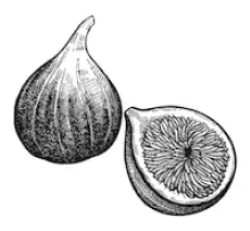
\includegraphics[width=1in,height=1.25in,clip,keepaspectratio]{figuras/author1.png}}]{Dafnh\^e Thor Castro de Martins Barros}
received the B.S. degree in Electrical Engineering. He is currently an M.Sc. candidate in Control and Automation Engineering with the Graduate Program in Control and Automation Engineering (PROPECAUT), Federal Institute of Esp\'irito Santo (IFES), Serra, Brazil. His research interests include real-time embedded systems, spaceborne computing architectures, compact thermal modeling, Model Predictive Control (MPC), and edge artificial intelligence in harsh aerospace environments.
\end{IEEEbiography}

\begin{IEEEbiography}[{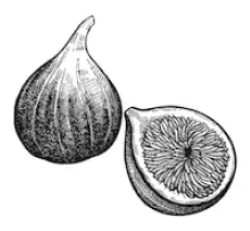
\includegraphics[width=1in,height=1.25in,clip,keepaspectratio]{figuras/author2.png}}]{Fl\'avio Barcelos Braz da Silva}
received the B.S., M.Sc., and Ph.D. degrees in Electrical Engineering. He is currently an Associate Professor with the Department of Control and Automation Engineering and a permanent faculty member of the Graduate Program in Control and Automation Engineering (PROPECAUT) at the Federal Institute of Esp\'irito Santo (IFES), Serra, Brazil. His research interests encompass robust and optimal control, space systems engineering, system identification, and embedded control.
\end{IEEEbiography}

\end{document}
